% Drawing 148/04-3 -- folder 148, batch 04, archive page 61 (PDF page 62).
% Transcription: ici un petit graphe : un sommet marqué $g$, d'où part vers le haut un faisceau d'arêtes libres, avec une accolade et « $\nu$ » au bout du faisceau.
% Kind: graph: one vertex of genus g with a bundle of nu legs. Method 2 (schematic redraw from the facsimile). Status: ok.
% Notes: Ink. One heavy vertex, the letter g under it, five legs fanning upwards (the number drawn stands for nu), a small brace and the letter nu to the right of their ends. Redrawn 2026-11-12 (issue 128): to check again.
% Coordinates: 1 unit = 1 mm = 1/100 of the crop width, y downwards as on the crop (bbox in page fractions: [0.4, 0.775, 0.58, 0.845]).
% Redrawn by Claude (claude-fable-5-2), issue #128, 2026-11-12; not checked by a human; not compiled (no TeX in the session).
% Rights: reproduces part of the work -- behind RENDER_TRANSCRIPTS, never published by itself.
\documentclass[tikz,border=3pt]{standalone}
\usepackage{amsmath,amssymb}
\usetikzlibrary{patterns,arrows.meta}
\tikzset{pencil/.style={black!45}, struck/.style={black!35}, mpt/.style={circle,draw,inner sep=1.3pt}, pt/.style={circle,fill,inner sep=0.9pt}, opt/.style={circle,draw,fill=white,inner sep=1.1pt}, Rd/.style={red!75!black}, Gn/.style={green!45!black}, Br/.style={brown!70!black}}
\begin{document}
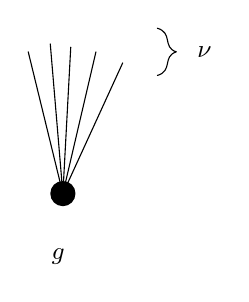
\begin{tikzpicture}[x=1mm,y=-1mm,line cap=round,line join=round,font=\small]
\coordinate (v) at (45,31);
\draw (v) -- (40.6,13);
\draw (v) -- (43.4,12);
\draw (v) -- (46,12.4);
\draw (v) -- (49.2,13);
\draw (v) -- (52.6,14.4);
\fill (v) circle [radius=1.6];
\node at (44.4,39) {$g$};
\draw (57,10) .. controls (59,10.6) and (57.6,12.4) .. (59.4,13) .. controls (57.6,13.6) and (59,15.4) .. (57,16);
\node at (63,13) {$\nu$};
\end{tikzpicture}
\end{document}
